\section{Referencia de la Clase List\-Provincias\-View}
\label{classListProvinciasView}\index{ListProvinciasView@{ListProvinciasView}}
Muestra y administra la ventana con la lista de provincias.  


{\tt \#include $<$listprovinciasview.h$>$}

Diagrama de colaboraci\'{o}n para List\-Provincias\-View:\begin{figure}[H]
\begin{center}
\leavevmode
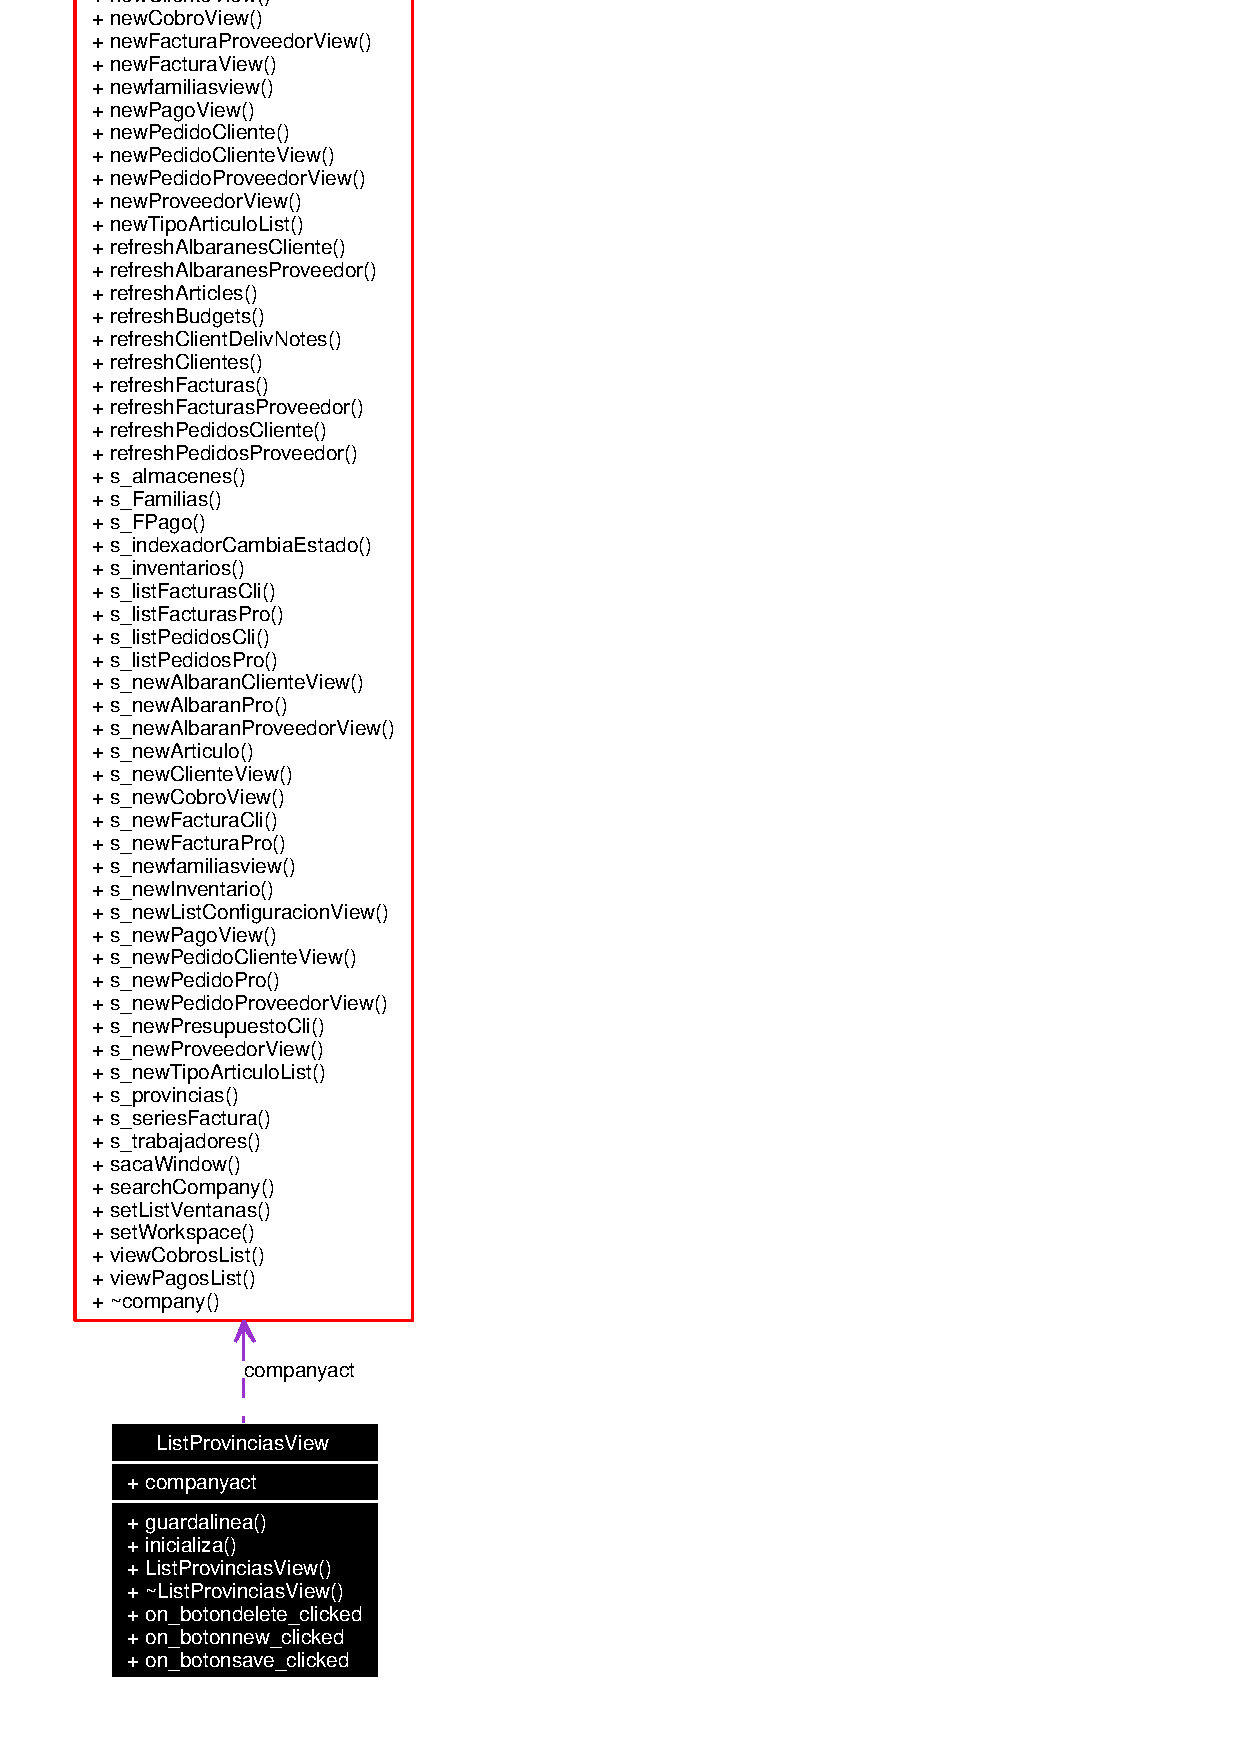
\includegraphics[width=99pt]{classListProvinciasView__coll__graph}
\end{center}
\end{figure}
\subsection*{Slots p\'{u}blicos}
\begin{CompactItemize}
\item 
virtual void {\bf on\_\-botondelete\_\-clicked} ()\label{classListProvinciasView_i0}

\item 
virtual void {\bf on\_\-botonnew\_\-clicked} ()\label{classListProvinciasView_i1}

\item 
virtual void {\bf on\_\-botonsave\_\-clicked} ()\label{classListProvinciasView_i2}

\end{CompactItemize}
\subsection*{M\'{e}todos p\'{u}blicos}
\begin{CompactItemize}
\item 
int {\bf guardalinea} (int)\label{classListProvinciasView_a0}

\item 
void {\bf inicializa} ()\label{classListProvinciasView_a1}

\item 
{\bf List\-Provincias\-View} ({\bf company} $\ast$, QWidget $\ast$parent=0)\label{classListProvinciasView_a2}

\end{CompactItemize}
\subsection*{Atributos p\'{u}blicos}
\begin{CompactItemize}
\item 
{\bf company} $\ast$ {\bf companyact}\label{classListProvinciasView_o0}

\end{CompactItemize}


\subsection{Descripci\'{o}n detallada}
Muestra y administra la ventana con la lista de provincias. 



La documentaci\'{o}n para esta clase fu\'{e} generada a partir de los siguientes archivos:\begin{CompactItemize}
\item 
listprovinciasview.h\item 
listprovinciasview.cpp\end{CompactItemize}
